%=====================================================================
\section{Why \ember{} Misses Quiet Concepts}
\label{sec:motivation}
%=====================================================================

\begin{figure*}[t]
  \centering
  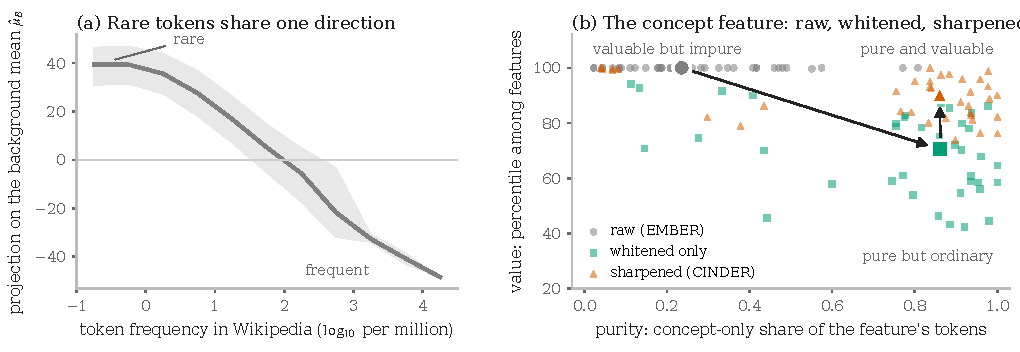
\includegraphics[width=\textwidth]{figures/mechanism.pdf}
  \caption{Why \ember{} misses quiet concepts, on Gemma-2-2B-it. (a)~Across the vocabulary, rarer tokens share a larger component along the background mean $\hat\mu_B$ (median and interquartile range per frequency bin); concept tokens are rarer than neutral ones in 35 of 38 concepts. (b)~A sparse feature seeded on each concept's lexicon tokens and run to its fixed point, per concept (small markers) with medians (large markers). In the raw matrix it is valuable but drifts to other rare tokens (impure); after whitening it is pure but ordinary; after sharpening it is pure and valuable.}
  \label{fig:mechanism}
\end{figure*}

A natural question is how reliably \ember{}'s first two stages find the target concept.
To study this, we reproduced \ember{} on Gemma-2-2B-it, matching the published accuracies within four points (\S\ref{app:ember}), and inspected each stage on its flagship concept, Harry Potter, before testing each observation on more concepts and seeds.
We find five issues, summarized in Table~\ref{tab:diagnosis}.

\paragraph{The concept hides behind rarity}
Sparse MF minimizes the squared reconstruction error, so a feature is worth the energy it explains along a group of aligned tokens.
Concept tokens are not low in energy (per token they carry as much as neutral tokens), but they are rare: across 38 concepts, concept-only tokens are rarer than neutral ones in \expnum{35} (median \expnum{9.4} vs.\ \expnum{12.9} per million words).
In Gemma's embeddings, rare tokens share a large component along the background mean $\mu_B$ (Figure~\ref{fig:mechanism}a), consistent with the degeneration of rare-token embeddings \citep{gao2019representation}.
The concept feature of \ember{}'s raw fit is therefore loud for the wrong reason: it sits at the \expnum{86th} percentile of feature norms, with \expnum{42\%} of its norm along $\hat\mu_B$ against \expnum{12\%} for a typical feature, and it groups the concept with unrelated rare tokens.
On Harry Potter (seed 42), its first 19 tokens are all Harry Potter, but further down sit Nestl\'e, Lego and Trump, which \ember{} would edit, among unrelated names and taxonomic suffixes (\S\ref{app:examples}).
Removing the shared component does not solve the problem: the concept's tokens then form a pure cluster, but an ordinary one, which the factorization finds less often than before (Figure~\ref{fig:mechanism}b; \S\ref{sec:analysis}).
In this sense the concept is \emph{quiet}.

\paragraph{One width does not fit all concepts}
\ember{} keeps the top 1\% of tokens in every feature, about 48 tokens.
Since concepts differ in breadth, a fixed width cuts a broad concept short and pads a narrow one with unrelated tokens.
To measure this, we re-solve the coefficients densely with the dictionary fixed and rank all tokens by their share of the concept feature; the \emph{natural tail} is the rank at which most of the next tokens stop being specific to the concept's page.
In \ember{}'s matrix the 1\% cut is too short for \expnum{15} of 38 concepts and too long for another \expnum{15} (\S\ref{app:gs}).

\paragraph{The judge loses the concept in its summary}
\ember{}'s judge does not see the feature, only a one-sentence description of its top tokens, and the description is where concepts get lost.
In our runs, \emph{heroin} was described as ``addictive drugs'' and \emph{World War II} as ``20th-century totalitarian regimes''; both were rejected, as was Valentine's Day, each at exactly the 0.85 confidence cutoff.
A rejected concept is not erased at all, since no feature is left to subtract: on 12 held-out concepts \ember{} edits nothing in \expnum{19 of 60} runs, and a multilingual \ember{} fit accepts a concept feature for only \expnum{10 of 38} concepts (\S\ref{sec:experiments}).

\paragraph{The edit stays in English}
\ember{} edits the rows of English tokens, and its authors leave other languages to future work.
We find that a concept erased in English largely survives in other languages: on Gemma, \ember{}-edited models retain \expnum{0.19--0.24} more of the concept's knowledge in German, Spanish, French and Russian than in English, and \expnum{0.31--0.41} more in Russian, whose tokens the English edit never touches (\S\ref{app:ml}).
The two obvious remedies both fall short.
Running \ember{} separately in every language multiplies the factorizations and judge calls by the number of languages, and a single \ember{} fit on multilingual text accepts a concept feature for only \expnum{10 of 38} concepts on Llama-3.1-8B.
In the multilingual matrix the concept is about \expnum{3} times quieter than in English, and the means of the eight languages carry \expnum{34} times the energy of the concept; the fit gives \expnum{14\%} of its candidate features to single languages (\S\ref{sec:exp-ml}).

\paragraph{The evaluation rewards destroying tokens}
\ember{} chooses the erasure strength $\delta$ by $H$ on validation questions.
In our reproduction, this selects the largest value, $\delta = 200$, for \expnum{6 of the 10} concepts \ember{} edits.
On Harry Potter, where the concept part $\cvec_t$ is about 0.6 of a token's length, the edited embedding is about 120 times longer than the original and points along $-\cvec_t$ (40--120 times across concepts): the word is replaced rather than cleaned.
None of the metrics registers this.
The concept questions contain the edited words, so a destroyed word counts as erased knowledge; the similar-domain questions avoid them, the MMLU gate never binds in any of the \expnum{344} grid points we scored, and Alpaca coherence stays at or above \expnum{0.92}.
Free text tells a different story: on Harry Potter at $\delta = 200$, \expnum{12 of 20} prompts that use the edited words in other senses break (asked about Prince Harry, the model describes the singer Prince), against \expnum{0--1 of 20} at $\delta = 1$.
We refer to this regime as \emph{token destruction}.

\begin{table}[t]
  \centering
  \small
  \setlength{\tabcolsep}{3pt}
  \begin{tabular}{@{}P{1.45cm}P{3.15cm}P{2.3cm}@{}}
    \toprule
    Stage & Issue & \cinder{}'s change \\
    \midrule
    Decompose & The concept hides behind rarity; once separated, it is quiet & Contrastive Sharpening (\S\ref{sec:cs}) \\
    Decompose & One width for every feature & Global Sparsity (\S\ref{sec:cs}) \\
    Identify & The judge reads a summary that loses the concept & Two-Way Judge (\S\ref{sec:twj}) \\
    Erase & Centred and uncentred edits differ by a direction all tokens share & Both variants (\S\ref{sec:cinderz}) \\
    Scope & Edits English tokens only; one multilingual fit finds few concepts & One fit for eight languages (\S\ref{sec:ml}) \\
    Evaluate & Destroying a word scores as erasing a concept & Collateral-aware evaluation (\S\ref{sec:setup}) \\
    \bottomrule
  \end{tabular}
  \caption{The issues we identify in each stage of \ember{} and the change \cinder{} makes. The erasure-stage row concerns a choice in our own design rather than an issue of \ember{}.}
  \label{tab:diagnosis}
\end{table}
